% Archivo generado automáticamente con los problemas
\section*{Problems}
Sección: 11_Spinor_solutions_and_CPT
Páginas: 220-223
Contenido:
11.1 In practice, we only rarely use explicit representations of the Dirac matrices. Most
calculations can be done using algebraic identities that depend only on {γμ, γν} =
2gμν. Derive algebraically (without using an explicit representation):
(a) (γ5)2 = 1
(b) γμ/pγμ = −2/p
(c) γμ/p/q/pγμ = −2/p/q/p
(d)
+
γ5, γμ,
= 0
(e) Tr[γαγμγβγν] = 4(gαμgβν −gαβgμν + gανgμβ)

11.2 Spinor identities.
(a) Show that 
sus(p)¯us(p) = /p + m and 
svs(p)¯vs(p) = /p −m.
(b) Show that ¯uσ(p)γμuσ′(p) = 2δσσ′pμ.

11.3 Prove that massless spin-1 particles coupled to spin-0 or spin- 1
2 particles imply a
conserved charge. You may use results from Section 9.5.

11.4 Show that for on-shell spinors
¯u(q)γμu(p) = ¯u(q)
qμ + pμ
2m
+ iσμν(qν −pν)
2m
u(p),
(11.92)
202
Spinor solutions and CPT
where σμν =
i
2[γμ, γν]. This is known as the Gordon identity. We will use this
when we calculate the 1-loop correction to the electron’s magnetic dipole moment.
Show that ¯uσ(p)γμuσ′ (p) = −iδσσ′ pμ
p0 .

11.5 Derive the charge-conjugation properties of the spinor bilinears in Eqs. (11.54) to
(11.56).

11.6 The physics of spin and helicity.
(a) Use the left and right helicity projection operators to show that the QED vertex
¯ψhγμψh′ vanishes unless h = h′.
(b) For the non-relativistic limit, choose explicit spinors for a spinor at rest. Show
that ¯ψsγμψs′ vanishes unless s = s′.
(c) Use the Schr¨odinger equation to show that in the non-relativistic limit the
electric field cannot flip an electron’s spin, only the magnetic field can.
(d) Suppose we take a spin-up electron going in the +z direction, and turn it around
carefully with electric fields so that now it goes in the −z direction but is still
spin up. Then its helicity flipped. Since all interactions between electrons and
photons preserve helicity, how can this have happened?
(e) How can you measure the spin of a slow electron?
(f) Suppose you have a radioactive source, such as cobalt-60, which undergoes β-
decay 60
27Co →60
28 Ni + e−+ ¯ν. How could you (in principle) find out if those
electrons coming out are polarized; that is, if they all have the same helicity?
Do you think they would be polarized? If so, which polarization do you expect
more of?

11.7 Show that the most general Lagrangian term you can write down in terms of Dirac
spinors, γ-matrices, and the photon field Aμ is automatically invariant under CPT.
To warm up, consider first the terms in Eq. (11.91).

11.8 Fierz rearrangement formulas (Fierz identities). It is often useful to rewrite spinor
contractions in other forms to simplify formulas. Show that
(a)
 ¯ψ1γμPLψ2
  ¯ψ3γμPLψ4

= −
 ¯ψ1γμPLψ4
  ¯ψ3γμPLψ2

(b)
 ¯ψ1γμγαγβPLψ2
  ¯ψ3γμγαγβPLψ4

= −16
 ¯ψ1γμPLψ4
  ¯ψ3γμPLψ2

(c) Tr

ΓMΓN
= 4δMN, with ΓM ∈{1, γμ, σμν, γ5γμ, γ5}
(d)
 ¯ψ1ΓMψ2
  ¯ψ3ΓNψ4

= 
P Q
1
16Tr

ΓP ΓMΓQΓN  ¯ψ1ΓP ψ4
  ¯ψ3ΓQψ2

where PL = 1−γ5
2
projects out the left-handed spinor from a Dirac fermion. The
identities with PL play an important role in the theory of weak interactions, which
only involves left-handed spinors (see Chapter 29).

11.9 The electron neutrino is a nearly massless neutral particle. Its interactions violate
parity: only the left-handed neutrino couples to the W and Z bosons.
(a) The Z is a vector boson, like the photon but heavier, and has an associated U(1)
gauge invariance (it is actually broken in nature, but that is not relevant for this
problem). If there is only a left-handed neutrino νL, the only possible mass
term of dimension four is a Majorana mass, of the form iMνT
Lσ2νL. Show that
this mass is forbidden by the U(1) symmetry.
This motivates the introduction of a right-handed neutrino νR. The most
general kinetic Lagrangian involving νL and νR is
Problems
203
Lkin = ν†
L¯σμ∂μνL + ν†
Rσμ∂μνR + m(ν†
LνR + ν†
RνL)
+ iM

νT
Rσ2νR −ν†
Rσ2ν⋆
R

,
(11.93)
where νL is a left-handed ( 1
2, 0) two-component Weyl spinor and νR is a right-
handed (0, 1
2) Weyl spinor. Note that there are two mass terms: a Dirac mass
m, as for the electron, and a Majorana mass, M.
(b) We want to figure out what the mass eigenstates are, but as written the
Lagrangian is mixing everything up. First, show that χL ≡iσ2ν⋆
R transforms
as a left-handed spinor under the Lorentz group, so that it can mix with νL.
Then rewrite the mass terms in terms of νL and χL.
(c) Next, rewrite the Lagrangian in terms of a doublet ⃗Θ ≡(νL, χL). This is not a
Dirac spinor, but a doublet of left-handed Weyl spinors. Using Lkin, show that
this doublet satisfies the Klein–Gordon equation. What are the mass eigenstates
for the neutrinos? How many particles are there?
(d) Suppose M ≫m. For example, M = 1010 GeV and m = 100 GeV. What are
the masses of the physical particles? The fact that as M goes up, the physical
masses go down, inspired the name see-saw mechanism for this neutrino mass
arrangement. What other choice of M and m would give the same spectrum of
observed particles (i.e. particles less than ∼1 TeV)?
(e) The left-handed neutrino couples to the Z boson and also to the electron
through the W boson. The W boson also couples the neutron and proton. The
relevant part for the weak-force Lagrangian is
Lweak = gW(ν†
L /WeL+e†
L /WνL)+gZ(ν†
L /ZνL)+gW (n /W ¯p+¯n /Wp). (11.94)
Using these interactions, draw a Feynman diagram for neutrinoless double β-
decay, in which two neutrons decay to two protons and two electrons.
(f) Which of the terms in Lkin and Lweak respect a global symmetry (lepton num-
ber) under which νL →eiθνL, νR →eiθνR and eL →eiθeL? Define
arrows on the e and ν lines to respect lepton number flow. Show that you
cannot connect the arrows on your diagram without violating lepton number.
Does this imply that neutrinoless double β-decay can tell if the neutrino has a
Majorana mass?

11.10 In Section 10.4, we showed that the electron has a magnetic dipole moment,
of order μB =
e
2me , by squaring the Dirac equation. An additional magnetic
moment could come from an interaction of the form B = iFμν ¯ψ[γμ, γν]ψ in the
Lagrangian. An electric dipole moment (EDM) corresponds to a term of the form
E = Fμν ¯ψγ5[γμ, γν]ψ.
(a) Expand the contribution of the electric dipole term to the Dirac equation
in terms of electric and magnetic fields to show that it does in fact give
an EDM.
(b) Which of the symmetries C, P or T are respected by the magnetic dipole
moment operator, B, and the EDM operator, E?

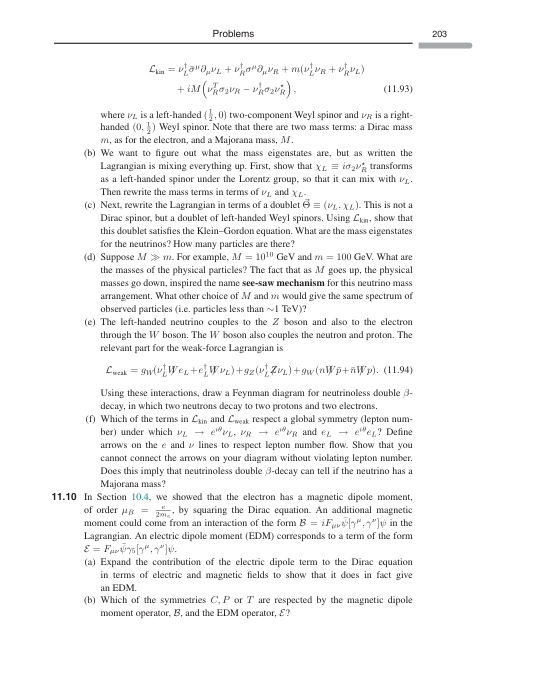
\includegraphics{./figs/11_Spinor_solutions_and_CPT_page_223.png}

---

